\section{Curso de DUNE/PDELab $2021$}

\begin{frame}[fragile]
	\frametitle{\secname}
	\framesubtitle{\url{https://dune-pdelab-course.readthedocs.io}}

	\begin{figure}[ht!]
		\centering
		\href{https://dune-pdelab-course.readthedocs.io}{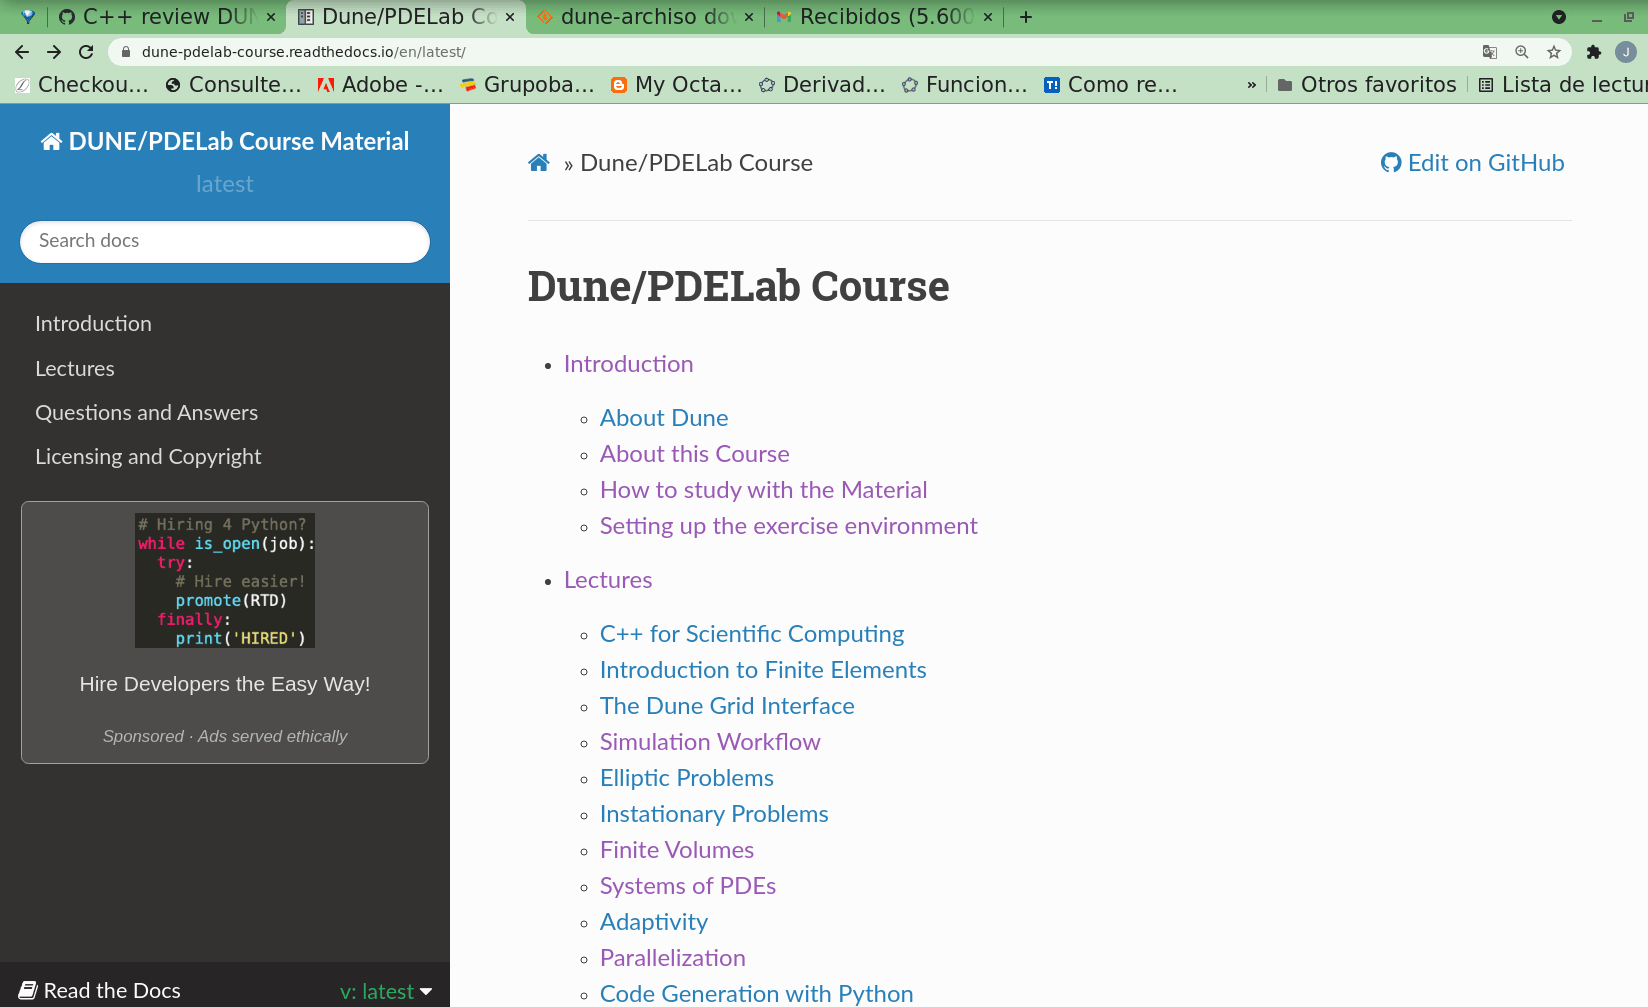
\includegraphics[height=8cm]{dune_course_2021}}
	\end{figure}
	\note{
		Cursos de DUNE anuales, lista de correo de preguntas y noticias.

		Cuenta con nueve tutoriales.
		El módulo se llama dune-pdelab-tutorials, \url{https://gitlab.dune-project.org/pdelab/dune-pdelab-tutorials}, es el sucesor de dune-grid-howto \url{https://gitlab.dune-project.org/core/dune-grid-howto}
	}
\end{frame}

\begin{frame}[fragile]
	\frametitle{Snippet en C++}
	\lstinputlisting[caption={Programa \texttt{dune-basics.cc}.},label=dune-basics.cc,]{dune-basics.cc}
	\note{
		Se muestra un código minimo de un programa basado en Dune.
		La forma de trabajo es importar las clases con las directivas %\lstinline|#include <dune/modulo/cabecera.hh>|

		\url{https://www.dune-project.org/sphinx/content/sphinx/dune-fem/mcf_nb.html}
		Es una simulación dinámica.
	}
\end{frame}

{
\usebackgroundtemplate{
	\centering
	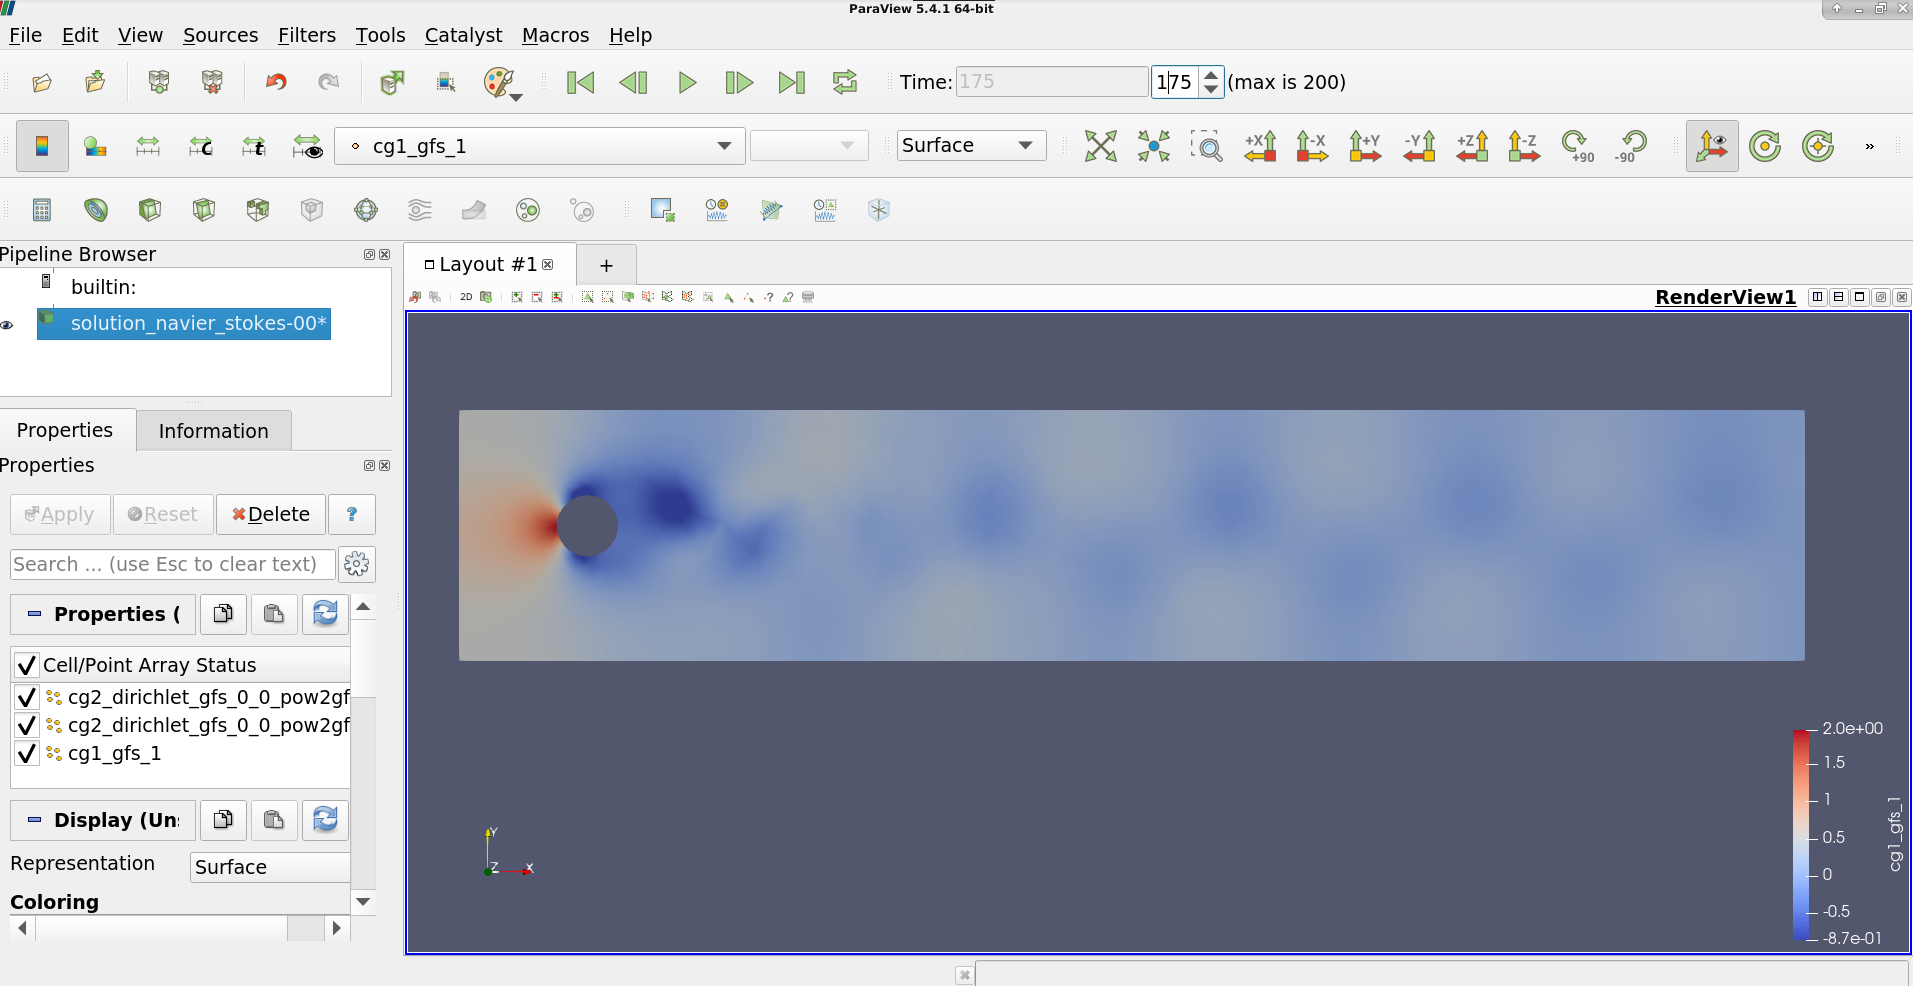
\includegraphics[width=\paperwidth]{tutorial-9}
}

\begin{frame}[plain]
	\note{
		Presentar el vídeo presenta la simulación de un flujo que obedece las ecuaciones de Navier Stokes, alrededor de un cilindro.
	}
\end{frame}
}
\begin{frame}[fragile]
	\frametitle{Snippet en Python}
	\begin{figure}[ht!]
		\centering
		\href{https://www.dune-project.org/sphinx/content/sphinx/dune-fem/mcf_nb.html}{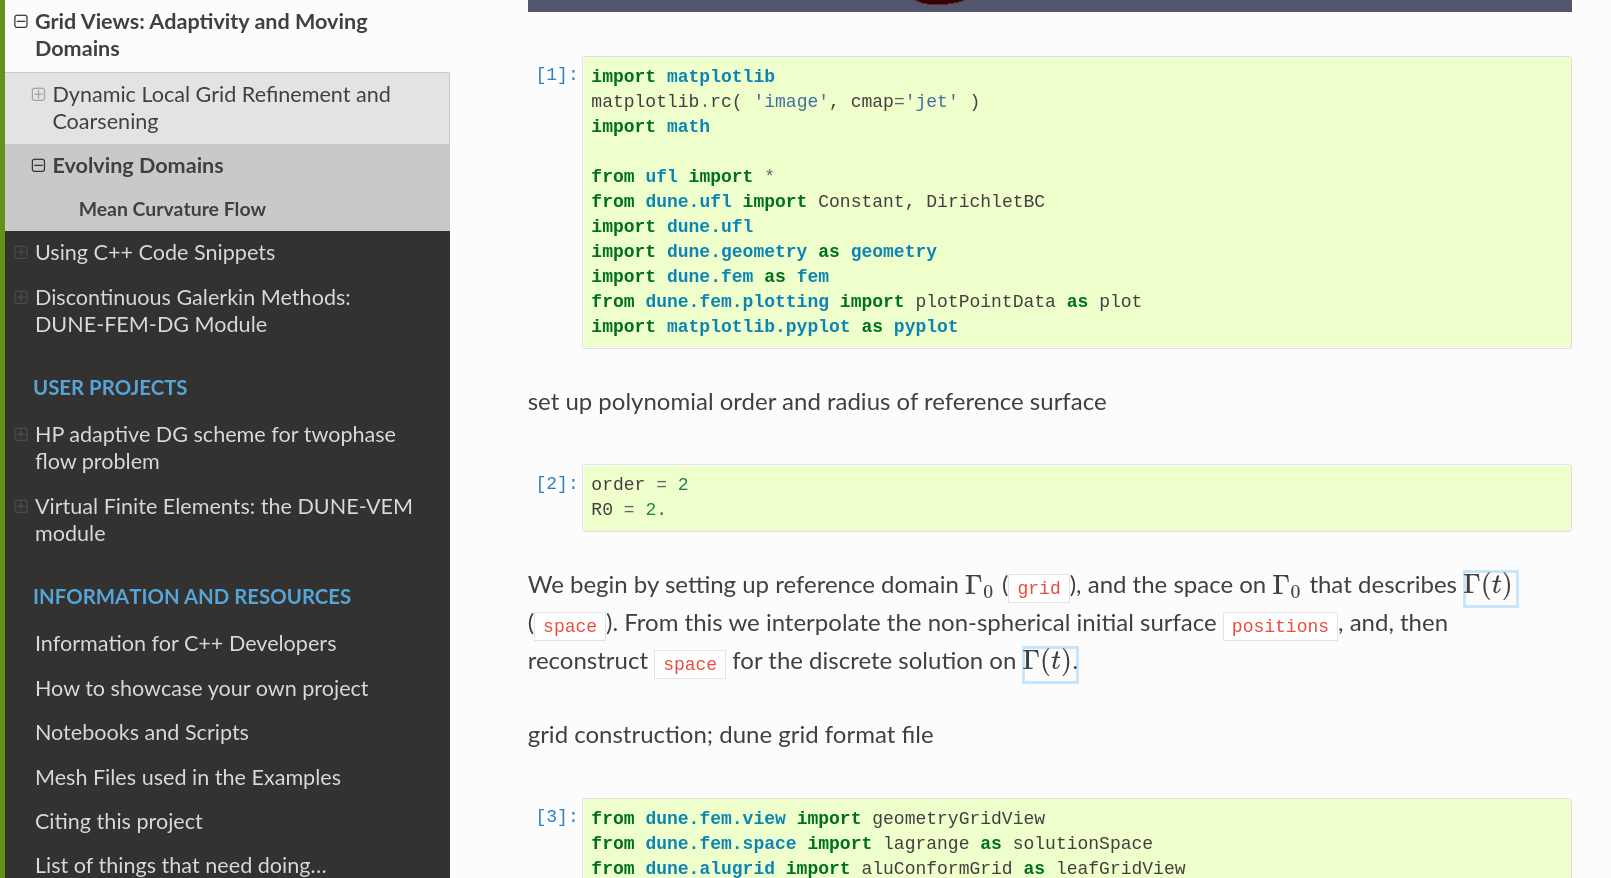
\includegraphics[height=8cm]{python_code}}
	\end{figure}

\end{frame}

{
\usebackgroundtemplate{\centering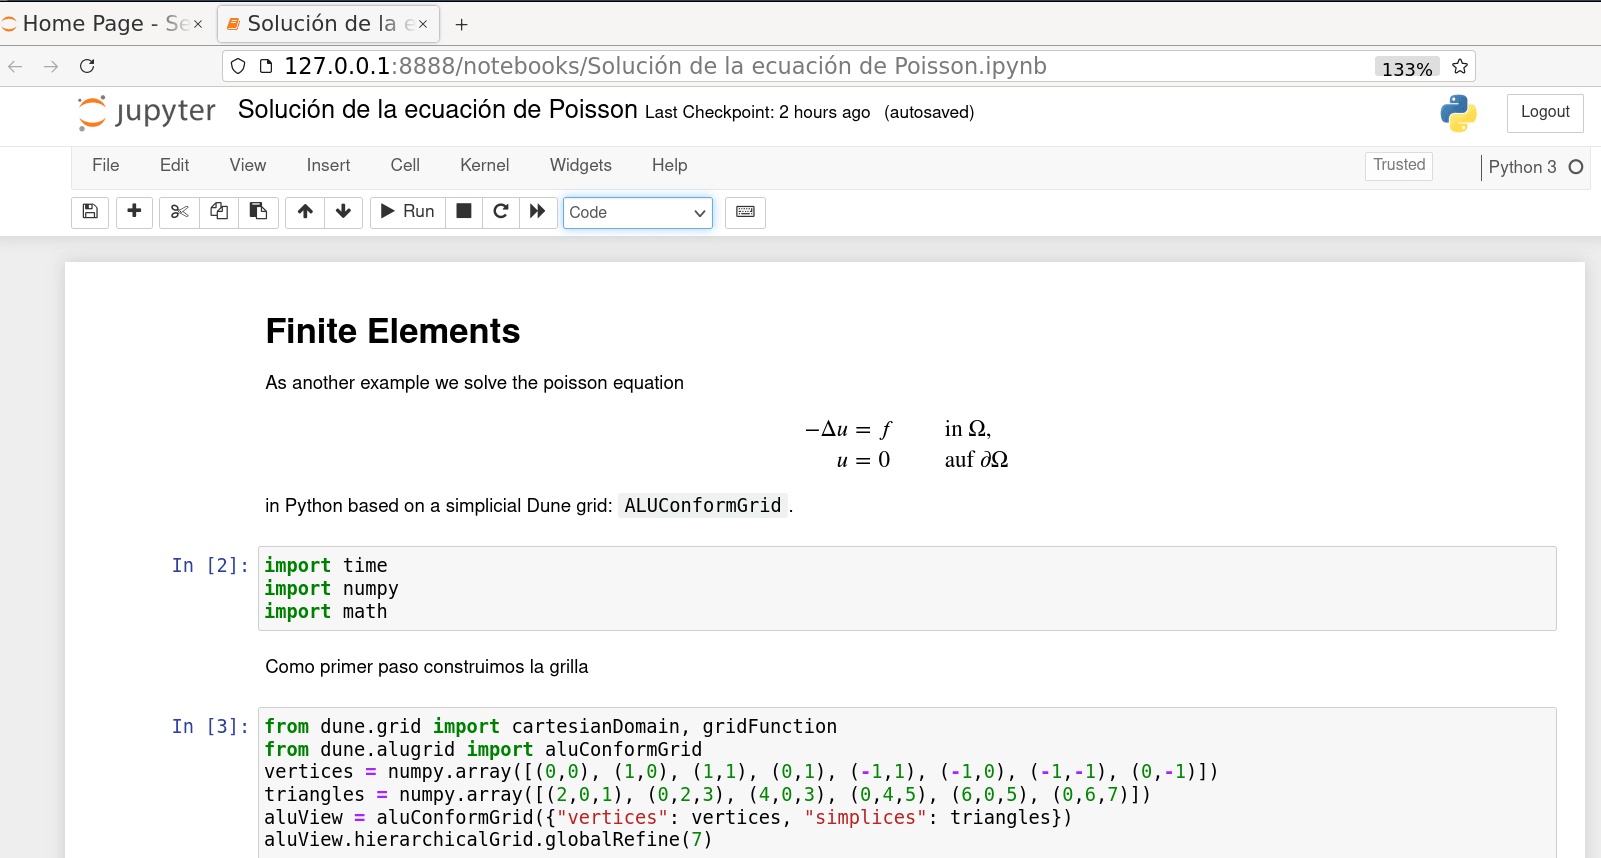
\includegraphics[width=\paperwidth]{jupyter01}}
\begin{frame}[plain]
	\note{
		Mostrar el artículo de dune-Python \url{https://arxiv.org/abs/1807.05252}, página 11.
		Los bindings de dune se encuentran en cada módulo, por ejemplo, dune-common, dune-geometry, dune-grid, dune-istl, etc, que depende de la instalación en C++ de dicho módulo.
	}
\end{frame}
}

{
\usebackgroundtemplate{\centering\href{https://github.com/cpp-review-dune}{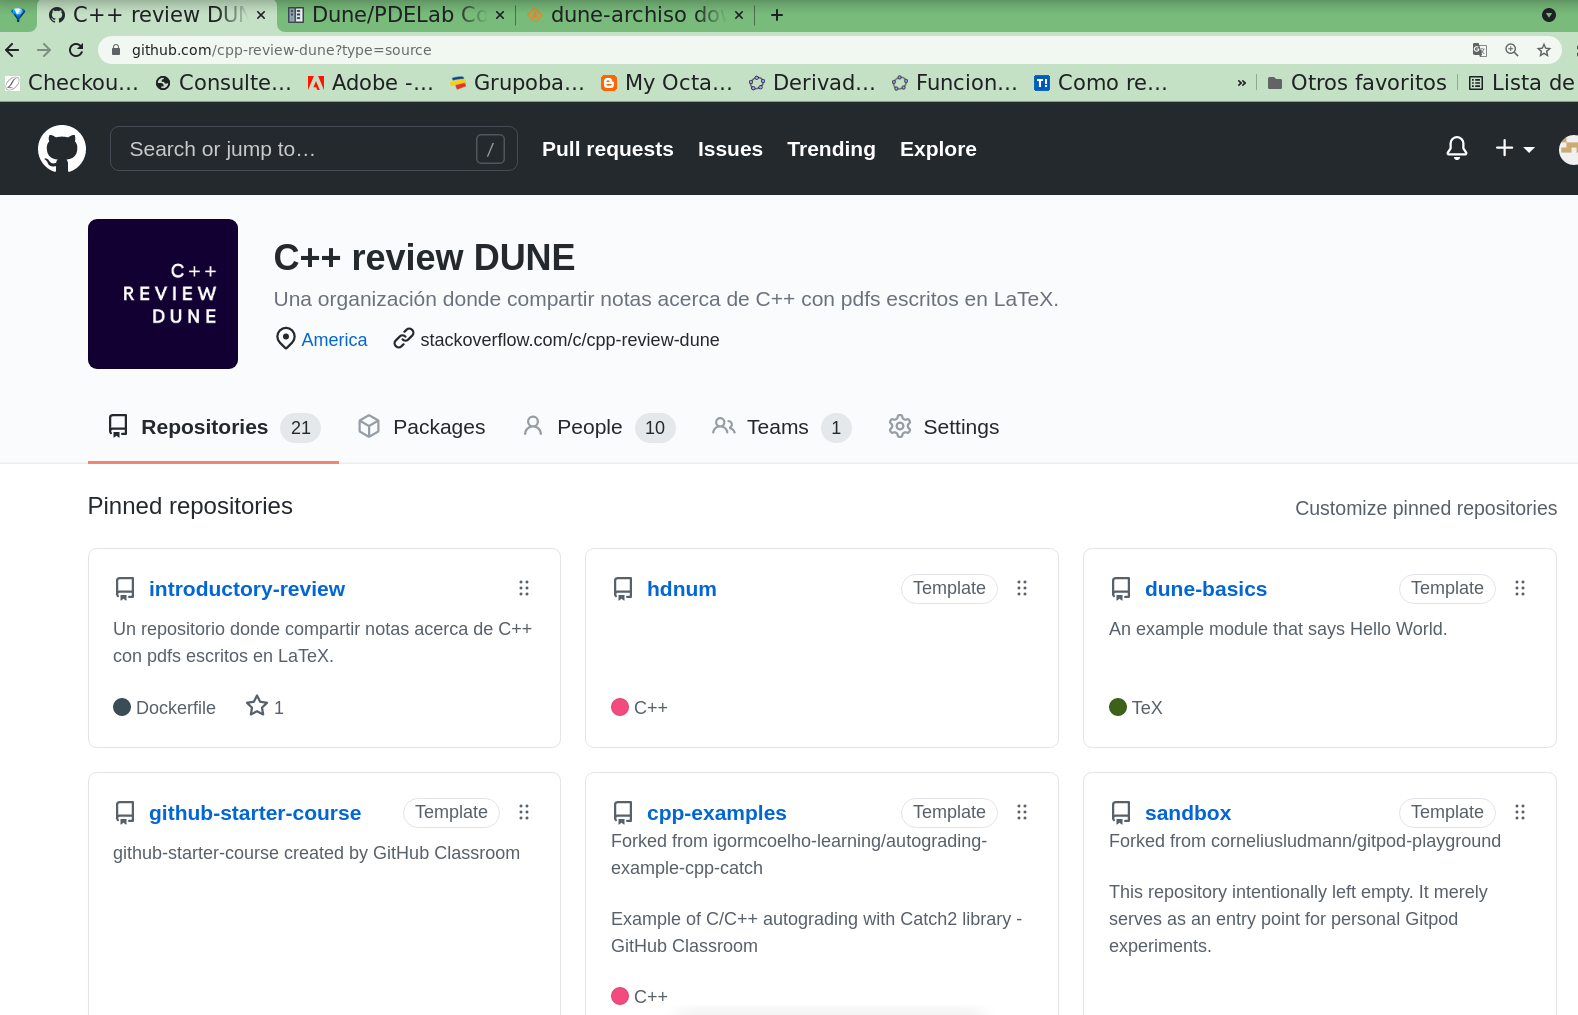
\includegraphics[width=\paperwidth]{cpp_review}}}
\begin{frame}[plain]
	\note{
		Página para repasar el curso virtual de DUNE/PDELab en el que contamos con los siguientes repositorios:
		\begin{itemize}
			\item \url{https://cpp-review-dune.github.io/introductory-review}
			      que contiene enlaces de interés y el enlace de acceso al grupo de Telegram. Además de otros cursos relacionados. Vídeos.
			\item Portar diversos módulos de DUNE en Arch Linux.
			\item La creación de imágenes Docker que permite la utilización de módulos específicos, incluidos la versión de Python, de manera periódica y automática, esto se puede ver en la sección de Actions en el repositorio introductory-review
			\item Por otro lado, han estado adoptando la metodología de Git en un proyecto de la Universidad Nacional de Colombia.
		\end{itemize}
	}
\end{frame}
}
